\capitulo{3}{Conceptos teóricos}

A continuación, se presentan aquellos conceptos que se han considerado necesarios para la comprensión de este trabajo:

\section{Contexto clínico y social}

\subsection{Nacimiento prematuro}
Según la Organización Mundial de la Salud (OMS), se considera prematuro a un recién nacido que nace antes de completar las 37 semanas de gestación. Este tipo de nacimiento se clasifica en tres categorías según la edad gestacional (EG) y según el peso al nacer \cite{who2023preterm}.

\begin{figure}[H]
    \centering
    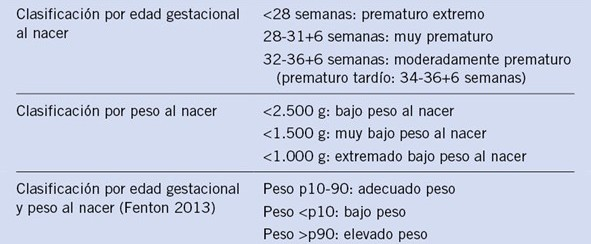
\includegraphics[width=0.75\linewidth]{img/EG.jpg}
    \caption{Clasificación de la prematuridad según la EG y el peso al nacer. Fuente: \cite{seneo2023protocolos}.}
    \label{fig:clasificación}
\end{figure}

La prematuridad representa el mayor desafío clínico actual de la Medicina Perinatal, siendo la principal causa de mortalidad infantil en menores de cinco años. La mayor parte de las complicaciones graves (morbimortalidad) se presenta en los recién nacidos “muy pretérminos”, cuya EG es inferior a 32 semanas y especialmente a los “prematuros extremos” \cite{rellan2008prematuro}.

\begin{figure}[H]
    \centering
    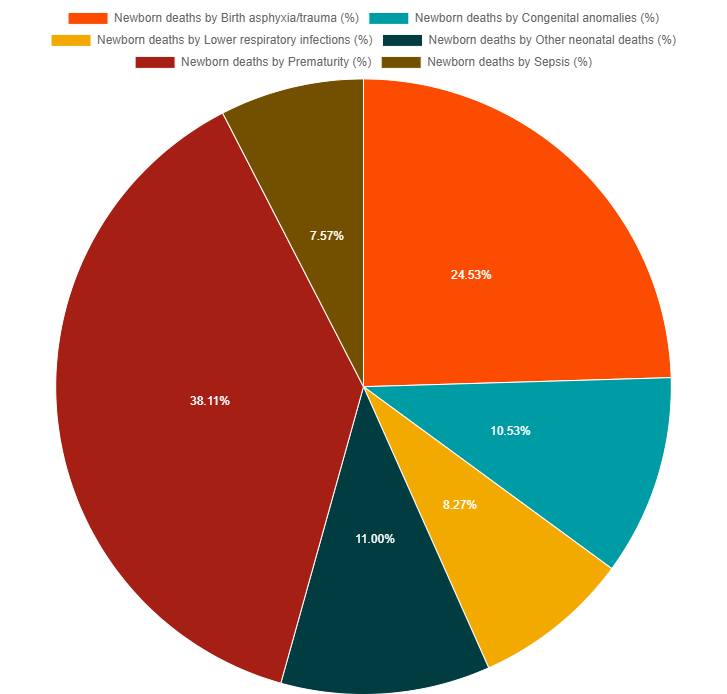
\includegraphics[width=0.7\linewidth]{img/causas.png}
    \caption{Principales causas de muerte infantil 2022 en todo el mundo 
    \\Fuente: \cite{hnn2024comprender}.}
    \label{fig:causas}
\end{figure}


Las tasas de supervivencia muestran diferencias significativas entre países: en naciones de bajos ingresos, alrededor del 50\% de los bebés nacidos a las 32 semanas o antes no sobreviven debido a la falta de atención adecuada y costo-eficaz, como el suministro de calor y el apoyo para la lactancia. En cambio, en países de altos ingresos, casi todos los bebés prematuros logran sobrevivir. Además, el uso ineficiente de la tecnología en países de ingresos medianos incrementa la discapacidad entre los recién nacidos prematuros que logran sobrevivir al período neonatal \cite{rios2017influencia}.

\subsubsection{Etiología} 

La mayor parte de los nacimientos prematuros ocurren debido a un parto prematuro espontáneo o a una amniorrexis prematura \footnote{rotura prematura de membranas}, representando más del 50\% de los casos. La presencia de infecciones clínicas o subclínicas es frecuente; de hecho, los cultivos fetales resultan positivos en el 60\% de los casos prematuros, frente al 20\% en los nacimientos a término. Entre las infecciones comunes se encuentran la vaginosis bacteriana y los niveles elevados de marcadores inflamatorios en el líquido amniótico. 

Otros factores de riesgo asociados a la prematuridad incluyen antecedentes de partos prematuros, condiciones socioeconómicas desfavorables, y el tabaquismo materno. La pobreza, el estrés materno, y el acceso limitado a la atención prenatal también son factores que incrementan el riesgo de un parto prematuro \cite{rellan2008prematuro}.

\subsubsection{Mortalidad en recién nacidos prematuros}

El riesgo de morbimortalidad está directamente relacionado con las semanas de gestación al nacer y con el peso (\ref{fig:Morbimortalidad}), pero también con el hecho de hacerlo en un lugar con el nivel asistencial adecuado \cite{COSTAS2005}.

\begin{figure}[H]
    \centering
    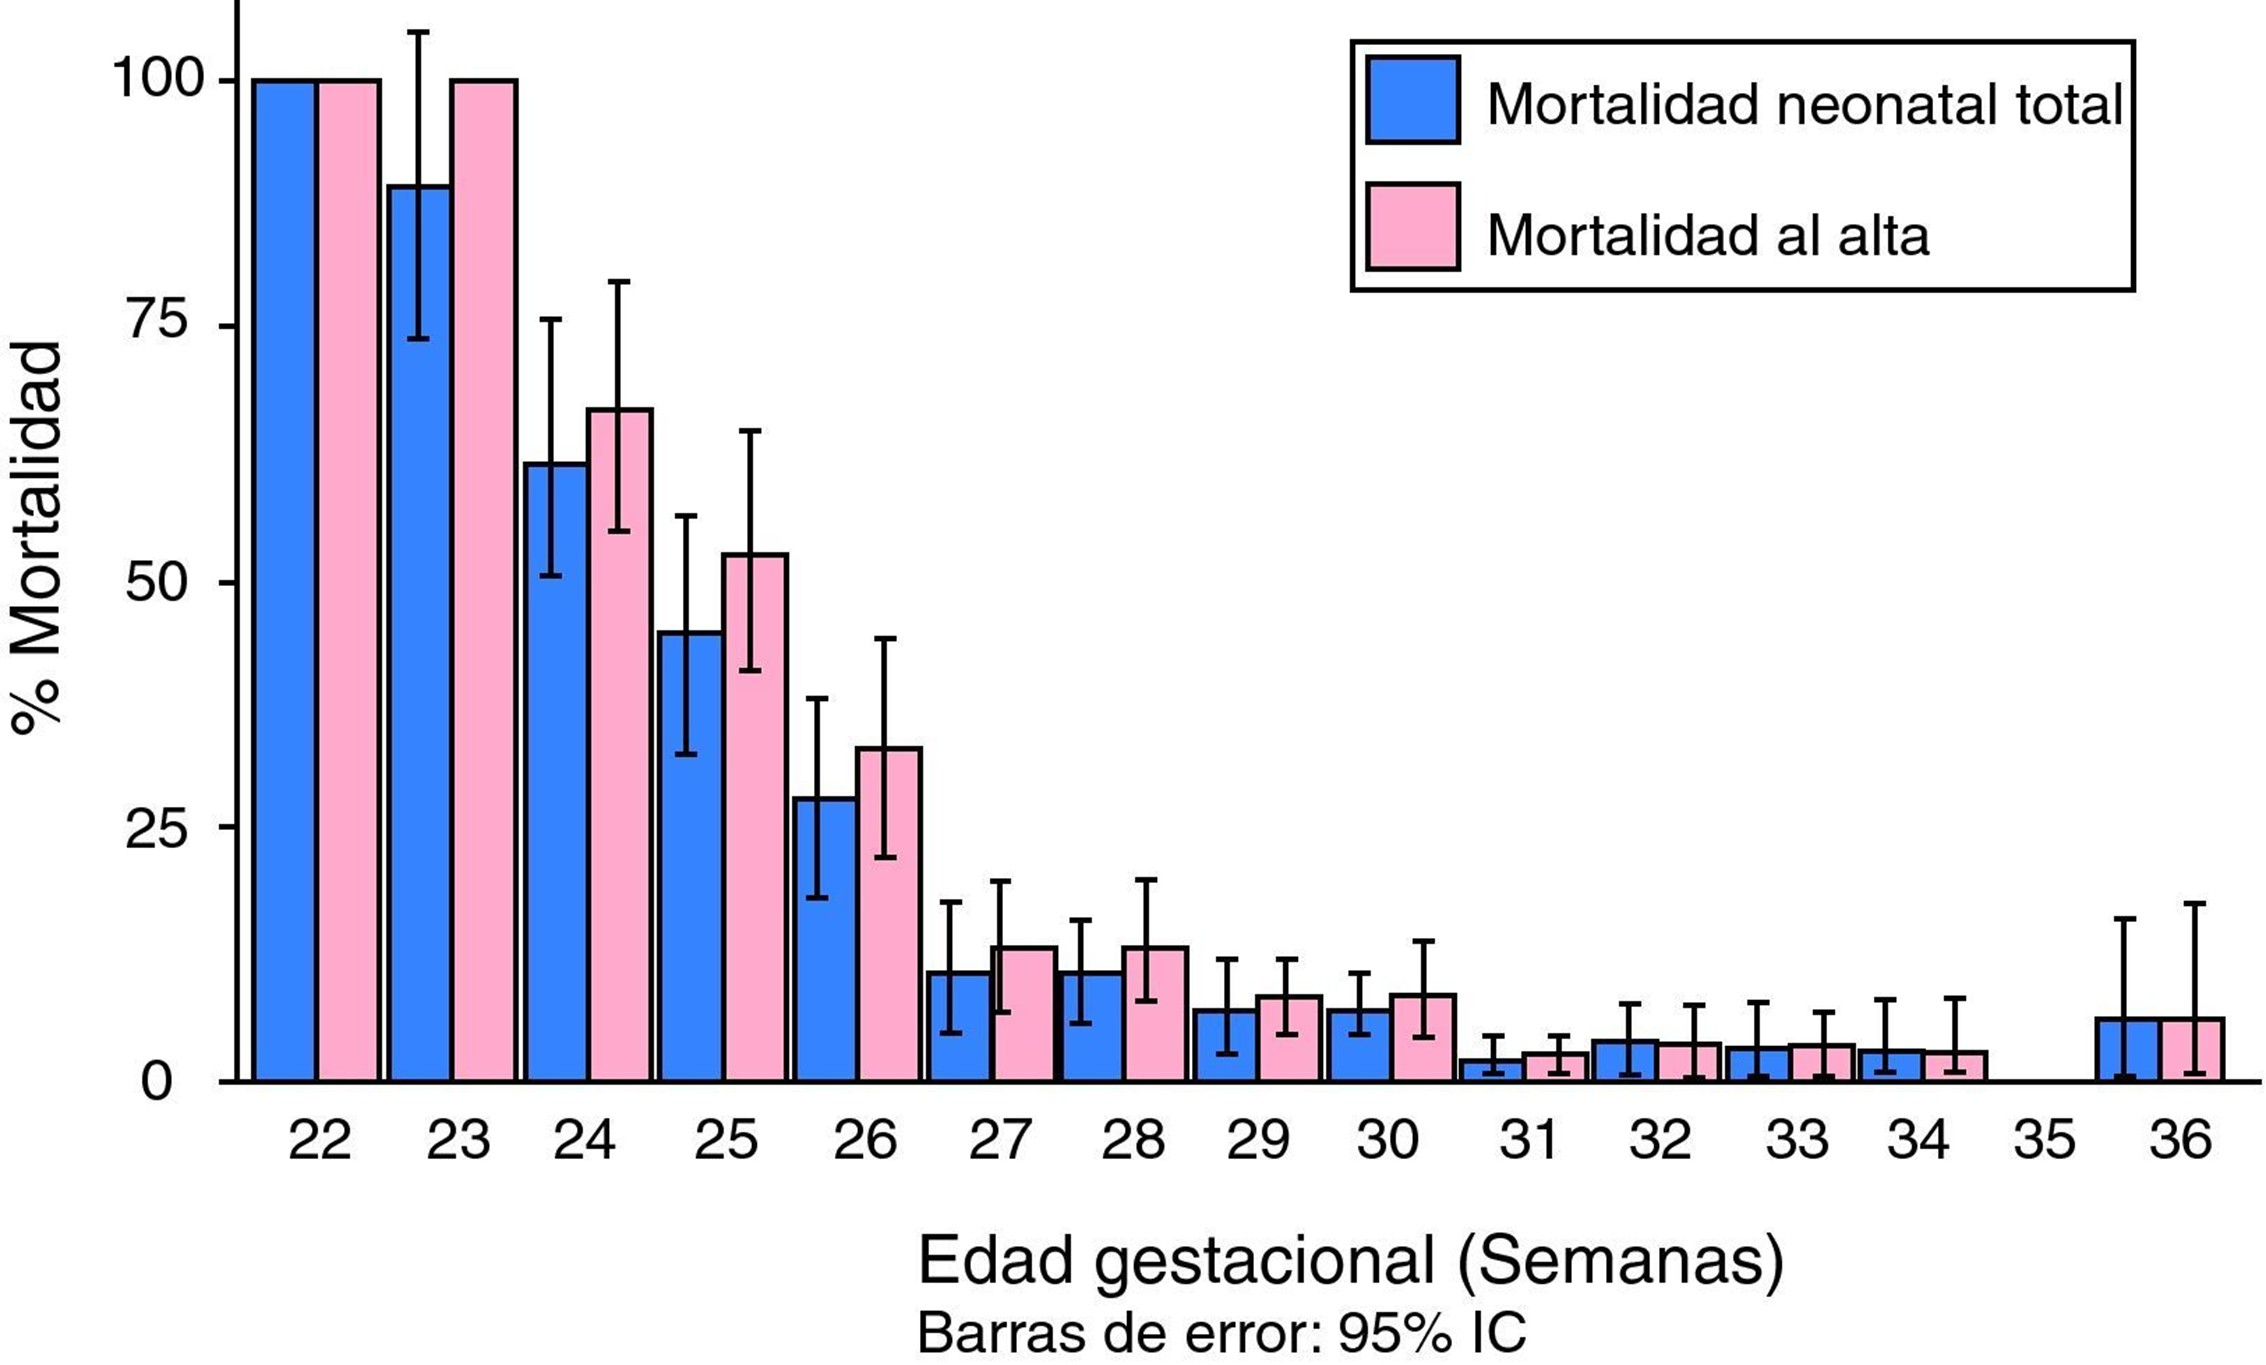
\includegraphics[width=0.7\linewidth]{img/Morbimortalidad.jpg}
    \caption{Representación de cómo se relaciona la morbimortalidad con el peso y la EG. Fuente: \cite{santesteban2012mortalidad}.}
    \label{fig:Morbimortalidad}
\end{figure}

Los recién nacidos prematuros enfrentan una serie de patologías debido a la inmadurez de sus órganos y sistemas, lo que genera una alta morbimortalidad y un motivo para que estos pacientes sean monitorizados de forma continua. A continuación, se enumeran algunas de las patologías más comunes junto con sus respectivos tratamientos:

\begin{itemize}
    \item \textbf{Patología Respiratoria:}
    Las complicaciones respiratorias son especialmente frecuentes, dado que los pulmones suelen estar poco desarrollados al momento del parto. Entre los problemas más comunes se encuentran:
    \begin{itemize}
        \item Enfermedad de Membrana Hialina (EMH): También conocida como síndrome de distrés respiratorio, esta patología está relacionada con el déficit de surfactante, una sustancia que evita el colapso de los alvéolos. El uso de CPAP (presión positiva continua en las vías respiratorias) es común para estabilizar a los bebés con esta condición
        \item Apnea del Prematuro: Los neonatos prematuros a menudo presentan episodios de apnea, donde dejan de respirar por periodos cortos de tiempo debido a la inmadurez de sus centros respiratorios en el cerebro. El monitoreo continuo de la saturación de oxígeno es importante para evitar este tipo de situaciones.
    \end{itemize}
    \item \textbf{Patología Neurológica: }El sistema nervioso central es vulnerable a la hipoxia y a las fluctuaciones hemodinámicas. Esto incrementa el riesgo de hemorragias intraventriculares (HIV) y leucomalacia periventricular\footnote{Lesión cerebral que afecta principalmente a bebés prematuros, caracterizada por la muerte o daño de la sustancia blanca alrededor de los ventrículos cerebrales.}. Se suele mantener un control preventivo de la oxigenación y la presión arterial, evitando cambios bruscos que puedan dañar el tejido cerebral.
    \item \textbf{Patología Cardiovascular: }Es frecuente que el conducto arterioso (una conexión que en la etapa fetal une la aorta con la arteria pulmonar) no se cierre después del nacimiento. Esta condición, conocida como persistencia del conducto arterioso (PCA), puede sobrecargar el sistema circulatorio y dificultar la oxigenación adecuada. Normalmente se intenta tratar con fármacos y, si no funciona, a veces hay que intervenir quirúrgicamente.
    \item \textbf{Patología Gastrointestinal:} El sistema digestivo en estos pacientes aún no está preparado para tolerar bien la nutrición, lo que incrementa el riesgo de enterocolitis necrotizante (EN), una afección grave que puede comprometer la integridad intestinal.
    \item \textbf{Inmunodeficiencia: }La incapacidad del recién nacido para contener una infección en un único órgano o sistema hace que, infecciones que en principio puedan estar controladas, sean sinónimo de una sepsis. 
\end{itemize}

Las patologías cuyos tratamientos no están mencionados no se consideran relevantes para el objetivo final de este trabajo \cite{rellan2008prematuro}.

\subsubsection{Epidemiología de la morbimortalidad}

La tasa de mortalidad infantil es uno de los indicadores más relevantes de la salud a nivel global, ya que proporciona información sobre las condiciones socioeconómicas en las que viven no solo los niños menores de 5 años, sino también el resto de la población, incluidos los adultos. Este indicador refleja, en particular, el estado de la atención perinatal, donde se observan diferencias significativas entre los países desarrollados y aquellos en vías de desarrollo.

Se relaciona con: el nivel socioeconómico, la salud materna, el acceso oportuno a los servicios de salud adecuados, la calidad en la atención y las políticas públicas en materia de salud materna y perinatal \cite{santesteban2012mortalidad}. También permite evaluar el estado de salud de las madres, las condiciones sanitarias e higiénicas, y las políticas de planificación familiar presentes en la región.

El Grupo Interinstitucional de las Naciones Unidas para la Estimación de la Mortalidad Infantil recopila y publica datos actualizados sobre la tasa de mortalidad infantil a nivel mundial, expresada en número de muertes por cada 1.000 nacidos vivos.  En la figura \ref{fig:epidemiologia} se representa la distribución de esta tasa por regiones:

\begin{figure}[H]
    \centering
    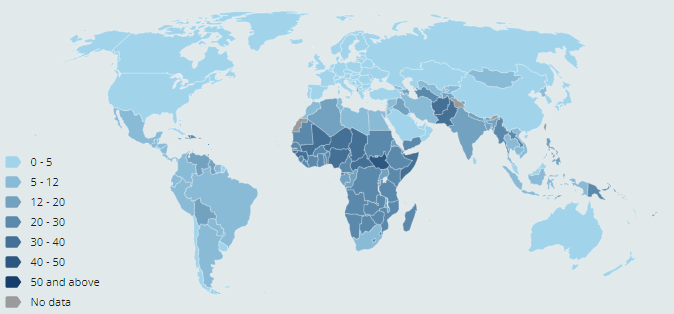
\includegraphics[width=0.9\linewidth]{img/epidemiologia.png}
    \caption{Tasa de mortalidad neonatal por cada 1.000 nacidos vivos (estimaciones globales más recientes). 
    \\ Fuente: \cite{unigme2024}.}
    \label{fig:epidemiologia}
\end{figure}

En las últimas décadas, ha habido importantes avances en la reducción de la mortalidad infantil, descendiendo un 51\% (de 37 muertes por cada 1000 nacidos vivos en 1990 a 18 en 2021) Actualmente, sobreviven más niños que nunca. Esto demuestra que es posible avanzar cuando se destinan suficientes recursos a la atención primaria de salud, lo que incluye la salud y bienestar infantiles.

Sin embargo, aún existen grandes desigualdades entre regiones y países. A nivel regional, África subsahariana y Asia meridional registran las tasas más altas de mortalidad neonatal, con 27 y 23 muertes por cada 1000 nacidos vivos, respectivamente, en 2021. Un bebé nacido en África subsahariana tiene diez veces más probabilidades de morir en su primer mes de vida que uno nacido en un país de ingresos altos, mientras que en Asia meridional ese riesgo es nueve veces mayor.


Dados todos estos datos estadísticos, es evidente que se necesita seguir invirtiendo en cuidados a los recién nacidos prematuros, sobre todo en aquellos lugares donde el acceso a los recursos se ve limitado.

\subsection{Tecnología aplicada a la prematuridad: La Incubadora neonatal}

La evidencia científica y los resultados de programas para reducir la mortalidad neonatal han permitido identificar intervenciones efectivas que, a corto y medio plazo, pueden tener un gran impacto en la supervivencia de los recién nacidos. 

Una de las soluciones más efectivas y consolidadas para abordar este problema ha sido la incubadora neonatal. Este dispositivo proporciona un entorno controlado y seguro para los recién nacidos que requieren cuidados adicionales, especialmente aquellos nacidos prematuramente o con condiciones de salud que los ponen en riesgo. 

Las incubadoras permiten recrear condiciones similares a las del vientre materno, favoreciendo que los bebés mantengan una temperatura estable y evitando que factores externos, como infecciones o cambios en la temperatura y la humedad, pongan en peligro su vida \cite{minsa2008prevencion}.

Este proyecto trabaja con una incubadora concreta,\textit{ In$^3$ator}, en cuyo diseño nos vamos a basar para explicar los tres componentes fundamentales de estos dispositivos (figura \ref{fig:partes_in3ator}):

\begin{itemize}
    \item \textbf{La cúpula o cubierta:} actúa como una barrera protectora, aislando al bebé del medio ambiente exterior. La cubierta debe permitir la visibilidad del bebé, por si hubiera problemas que las mediciones no perciben, pero que sí se pudieran apreciar a simple vista.
    \item \textbf{El chasis:} consiste en una base metálica que alberga los componentes electrónicos, como la fuente de energía, los sensores y los sistemas de soporte vital. Sobre él se coloca el porta colchón. 
    \item \textbf{El sistema de control de variables:} es responsable de monitorear y regular las condiciones internas, muy importantes para la estabilidad y recuperación del neonato:
    \begin{itemize}
        \item \textbf{Control térmico}: Los prematuros, debido a su bajo peso, piel fina y escasa grasa subcutánea, pierden calor con facilidad. Las incubadoras solucionan estas pérdidas mediante sistemas de calefacción por convección que controlan el aire que rodea al bebé. Existen dos modos de funcionamiento: uno regula la temperatura del aire de la cámara y otro, que se basa en la temperatura medida directamente en la piel del neonato.
        \item \textbf{Control de humedad}: El aire caliente circulante para el control de la termorregulación del neonato puede deshidratar al paciente, resecando su piel y sus mucosas, lo que favorece las infecciones. Para evitarlo, las incubadoras incluyen un sistema de humidificación que mantiene la humedad relativa en valores entre el 60\% y el 90\% \cite{restrepo2007incubadora}.
    \end{itemize}
\end{itemize} 

\begin{figure}[H]
    \centering
    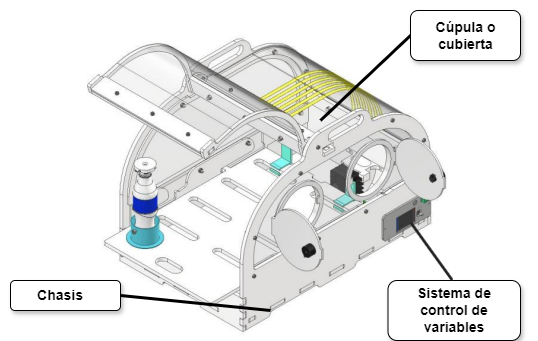
\includegraphics[width=0.65\linewidth]{img/partes_in3ator.png}
    \caption{Partes principales mencionadas de la incubadora \textit{In$^3$ator}. 
    \\ Fuente adaptada:\cite{in3es2025}. }
    \label{fig:partes_in3ator}
\end{figure}

Actualmente, la mayoría de las incubadoras modernas incluyen de forma integrada el control fisiológico del neonato a través de monitores multiparamétricos. 

De hecho, en los cuidados intensivos neonatales, la pulsioximetría se ha convertido en una herramienta importante, que aporta mucha información sobre el estado del paciente. Incorporar esta tecnología en la incubadora \textit{In$^3$ator} supone una mejora adicional, especialmente en entornos con recursos sanitarios limitados.

El siguiente bloque desarrolla los fundamentos sobre los que se basa esta tecnología y su aplicabilidad dentro del proyecto.


\section{Pulsioximetría}

La pulsioximetría es un procedimiento médico diseñado para medir la saturación de oxígeno en la sangre arterial (SaO$_2$), es decir, el porcentaje de hemoglobina que transporta oxígeno. Además, esta técnica permite cuantificar la frecuencia cardíaca y la amplitud del pulso.

\subsection{Fundamentos fisiológicos}

A continuación se describe en detalle la base fisiológica que utiliza la técnica y de dónde provienen los parámetros que mide:

\subsubsection{Sistema Cardiovascular}

El sistema cardiovascular, también conocido como sistema circulatorio, es uno de los sistemas vitales del cuerpo humano. Se encarga de transportar sangre, nutrientes, oxígeno, hormonas y de eliminar desechos metabólicos, a través de una extensa red de vasos sanguíneos y órganos especializados, siendo el corazón el protagonista de este proceso. 

El corazón, ubicado en la cavidad torácica y protegido por el pericardio, actúa como una potente bomba muscular. Su estructura se organiza en cuatro cavidades: dos aurículas y dos ventrículos. Las aurículas reciben la sangre; la aurícula derecha recoge la sangre desoxigenada proveniente del cuerpo a través de las venas cavas, mientras que la aurícula izquierda recibe la sangre oxigenada de los pulmones a través de las venas pulmonares. Posteriormente, los ventrículos se encargan de impulsar la sangre: el ventrículo derecho envía la sangre a los pulmones para que se oxigene, mientras que el ventrículo izquierdo bombea la sangre oxigenada hacia el resto del organismo a través de la aorta. Esta disposición garantiza una separación funcional entre la circulación pulmonar y la sistémica (figura \ref{fig:ciruclacion}), permitiendo que cada sistema cumpla su función de manera eficiente. 

\begin{figure}[H]
    \centering
    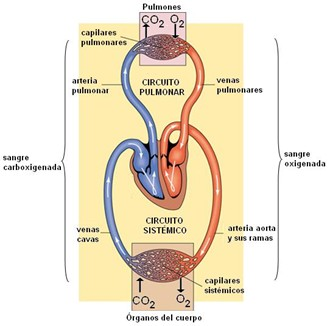
\includegraphics[width=0.55\linewidth]{img/ciruclacion.jpg}
    \caption{Representación de la circulación pulmonar y sistémica. Fuente: \cite{genomasur_cap13}.}
    \label{fig:ciruclacion}
\end{figure}

Además de su función de transporte, el sistema cardiovascular participa en la regulación de la temperatura corporal, el equilibrio de líquidos y electrolitos, y en la respuesta a las demandas metabólicas del organismo. Estos procesos se ajustan mediante la acción del sistema nervioso autónomo y diversas señales hormonales, lo que permite que el flujo sanguíneo se adapte de forma dinámica a las diferentes necesidades del cuerpo, ya sea en reposo o durante la actividad física \cite{kenhub2025}.\\



\subsubsection{Transporte del oxígeno en sangre }
El transporte de oxígeno es un proceso que garantiza el buen funcionamiento de los sistemas que componen el organismo. El oxígeno es indispensable para el metabolismo celular, ya que se utiliza en la respiración celular para generar energía en forma de adenosín trifosfato (ATP). Este proceso comienza con la inspiración de aire y culmina con la entrega de oxígeno a las células y tejidos a través del sistema circulatorio.\\ 

En la parte superior del sistema respiratorio, se encuentran la fosa nasal y la faringe, que conforman el sistema respiratorio superior. Estos órganos actúan como la primera línea de defensa, acondicionando el aire al filtrarlo, humidificándolo y calentándolo antes de que continúe su trayecto hacia el interior del aparato respiratorio. A partir de la laringe, el aire es conducido por la tráquea, la cual se ramifica en los bronquios y estos en bronquiolos, estructuras que componen el sistema respiratorio inferior. Este tramo se encarga de transportar el aire hasta los pulmones, donde se encuentran los alvéolos \cite{kenhubSistemasCuerpo2025}. \\

Cuando el aire entra en los pulmones y llega a los alvéolos pulmonares, el oxígeno se difunde a través de la membrana alveolar y se une a la hemoglobina, una proteína presente en los glóbulos rojos con gran afinidad por este gas. Cada molécula de hemoglobina puede transportar hasta cuatro moléculas de oxígeno, lo que permite una eficiente distribución a los tejidos.  \\

\begin{figure}[H]
    \centering
    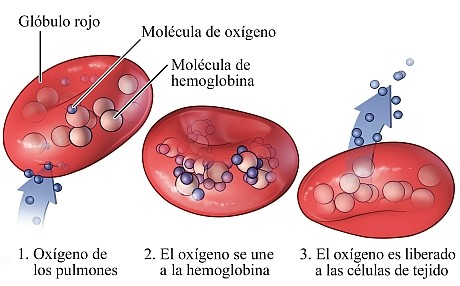
\includegraphics[width=0.6\linewidth]{img/hb.jpg}
    \caption{Transporte de oxígeno en sangre a través de la hemoglobina oxigenada. Fuente: \cite{cigna_hemoglobina}.}
    \label{fig:hb}
\end{figure}

Una vez que la sangre oxigenada llega a los tejidos a través de la circulación sistémica, los glóbulos rojos liberan el oxígeno, que difunde hacia las células. En su interior, el oxígeno es utilizado por las mitocondrias durante la fosforilación oxidativa, proceso mediante el cual se produce ATP, la principal fuente de energía celular. \\


\subsubsection{Parámetros fisiológicos relevantes en pulsioximetría}
Dado que la distribución de oxígeno depende de la eficiencia del transporte sanguíneo, es necesario medir ciertos parámetros fisiológicos para evaluar el estado hemodinámico y de oxigenación del organismo.

\newpage

\textbf{Frecuencia cardíaca}

La frecuencia cardíaca es uno de los signos vitales o indicadores más importantes para estimar la salud del cuerpo humano. Se trata del número de latidos que el corazón registra cada minuto, es decir, las veces que el corazón se contrae durante este tiempo \cite{enfermeriaCardiologia2025}.   

Varía a lo largo del día y de la noche y en respuesta a diferentes estímulos, como la actividad física, las amenazas o las emociones, por lo que su medición tiene gran variabilidad \cite{fundacionCorazon2025}.

Como norma general, la frecuencia normal en reposo de un adulto sano oscila entre 60 y 100 latidos por minuto (BPM); sin embargo, los recién nacidos tienen una frecuencia cardíaca elevada, oscilando entre 120 y 160 BPM, dado que la actividad de su organismo es muy intensa. 


\textbf{Saturación de Oxígeno (SaO$_2$)}

La hemoglobina, presente en los glóbulos rojos, se enlaza con el oxígeno en los alvéolos pulmonares para formar oxihemoglobina, que luego transporta el oxígeno a los tejidos donde se libera para ser utilizado por las células. Una vez liberado el oxígeno, la hemoglobina en su forma desoxigenada puede unirse al dióxido de carbono y llevarlo de vuelta a los pulmones para su eliminación durante la exhalación.  

La saturación de oxígeno (\ref{eq:sao2} o \ref{eq:sao2_2}) es el parámetro que se utiliza para expresar la cantidad de oxihemoglobina (HbO$_2$) respecto a la hemoglobina total (HbO$_2$ + Hb) que hay presente en nuestro organismo; es decir, describe el grado de capacidad de transporte del oxígeno en sangre \cite{gonzalez2019pulsioximetro}.

Se puede expresar como:

\begin{equation}
    SaO_2 = \frac{HbO_2}{HbO_2 + Hb} = \frac{c_{HbO_2}}{c_{HbO_2} + c_{Hb}}
    \label{eq:sao2}
\end{equation}

\begin{equation}
    SaO_2(\%) = \frac{HbO_2}{HbO_2 + Hb} \times 100\% = \frac{c_{HbO_2}}{c_{HbO_2} + c_{Hb}} \times 100\%
    \label{eq:sao2_2}
\end{equation}

\begin{center}
    Fuente: \cite{Alarco2015}.
\end{center}

En un adulto sano, los valores normales de saturación fluctúan entre el 95-100\%. Valores por debajo del 95\% (en reposo) se asocian con situaciones patológicas y del 92\% al 90\% con insuficiencia respiratoria crónica previa. En cambio, los valores normales de saturación de oxígeno en neonatos oscilan entre el 91\% y el 95\% \cite{vento2014oxigenoterapia}. 


Medir la saturación de oxígeno ayuda a evaluar la eficiencia del transporte de oxígeno y el funcionamiento pulmonar, ya que indica el grado de eficacia de un paciente en su respiración y cómo el oxígeno está siendo transportado a través del cuerpo \cite{weinmannEmergency2025}.

\subsection{Principios Físicos de la Medición Óptica }

La pulsioximetría se basa en una serie de principios físicos y ópticos que permiten estimar los parámetros fisiológicos a través de la interacción de la luz con los tejidos:


\subsubsection{Ley de Beer-Lambert}

La ley de Beer-Lambert fue descubierta independientemente (y de distintas maneras) por Pierre Bouguer en 1729, Johann Heinrich Lambert en 1760 y August Beer en 1852. Es una descripción empírica que relaciona la absorción de la luz con las propiedades del material que atraviesa \cite{Gilsanz2023}.

Describe cómo la intensidad de la luz que pasa a través de un medio absorbente disminuye en función de la concentración de la sustancia absorbente, la longitud del trayecto de la luz a través del medio, y el coeficiente de absorción específico de esa sustancia. Se puede expresar de dos maneras:

En su forma logarítmica (\ref{eq:ley_beer}), como absorbancia:

\begin{equation}
    A = \varepsilon \cdot b \cdot C 
    \label{eq:ley_beer}
\end{equation}


\begin{itemize}
    \item A es la absorbancia.
    \item $\varepsilon$ es el coeficiente de absorción (o extinción) del cromóforo\footnote{Un cromóforo es una parte de una molécula que absorbe luz visible o UV, lo que le da a la molécula un color.}
    \item b es la longitud del camino recorrido por la luz. 
    \item c es la concentración de las especies absorbentes. 
\end{itemize}

\newpage

O en forma exponencial (\ref{eq:ley_beer2}), como transmisión de luz:

\begin{equation}
    I = I_0 a^{-\mu \dot{d}} 
    \label{eq:ley_beer2}
\end{equation}

\begin{itemize}
    \item I= Intensidad de luz después de atravesar el medio.
    \item I$_0$ = Intensidad de luz inicial.
    \item $\mu$ = Coeficiente de atenuación. 
    \item d = Longitud del camino óptico.
\end{itemize}


\begin{figure}[H]
    \centering
    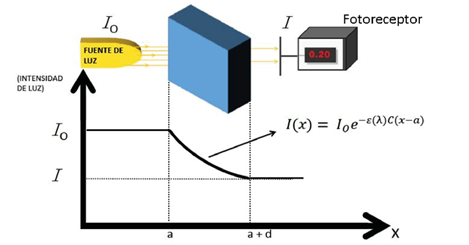
\includegraphics[width=0.75\linewidth]{img/beerlambert.png}
    \caption{Transmisión de luz a través de un medio absorbente según la Ley de Beer-Lambert. 
    \\ Fuente: \cite{Cordido2023}.}
    \label{fig:beerlambert}
\end{figure}

Ambas expresiones muestran que cuanto más absorbente es el medio, menos luz llegará al sensor, lo que permite estimar la concentración del compuesto de interés. 

En el caso de la pulsioximetría, el medio absorbente es el tejido del paciente, y el compuesto de interés es la hemoglobina, en sus dos formas: oxigenada (HbO$_2$) y reducida (Hb). Los tejidos biológicos y la sangre absorben luz en diferentes proporciones, y la hemoglobina es el principal cromóforo en la sangre que absorbe en el rango visible e infrarrojo cercano.

\begin{itemize}
    \item HbO$_2$ absorbe más luz en la región infrarroja (910–940 nm).
    \item Hb absorbe más luz en la región roja (640–660 nm).
\end{itemize}

\begin{figure}[H]
    \centering
    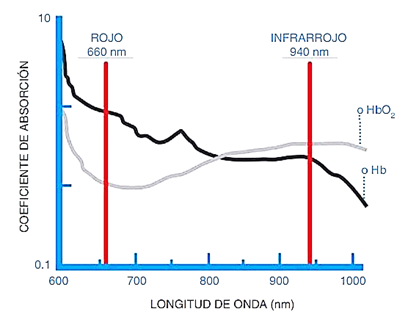
\includegraphics[width=0.6\linewidth]{img/absorbancia.png}
    \caption{Absorción de la hemoglobina y la oxihemoglobina en dos longitudes de onda. Fuente: \cite{DeLaPena2017}.}
    \label{fig:absorbancia}
\end{figure}

Por eso, los pulsioxímetros utilizan dos longitudes de onda distintas: una roja y otra infrarroja. Al medir cuánta luz de cada tipo atraviesa el tejido, el dispositivo puede calcular la proporción entre ambas formas de hemoglobina. 


\subsubsection{Señal de Fotopletismografía}

La fotopletismografía (PPG) es una técnica óptica utilizada para medir los cambios en el volumen sanguíneo mediante la detección de variaciones en la absorción de luz. Esta técnica es la base de funcionamiento de un pulsioxímetro. 

El principio de la PPG se basa en la emisión de luz a través de un transductor, que atraviesa los tejidos del paciente y es captada por un fotodetector. La cantidad de luz absorbida varía en función de los cambios en el volumen sanguíneo en los vasos, de acuerdo con la ley de Beer-Lambert, lo que permite registrar una señal que puede ser procesada para extraer información fisiológica relevante.

La señal obtenida mediante PPG presenta dos componentes principales: 

\begin{itemize}
    \item \textbf{Componente pulsátil o corriente alterna (AC): }Representa las variaciones periódicas asociadas con el ciclo cardíaco, directamente vinculadas con el volumen de sangre arterial impulsado por el corazón. Esta componente permite calcular la frecuencia cardíaca. 
    \item \textbf{Componente no pulsátil o corriente continua (DC): }Se debe a la absorción de luz por los tejidos circundantes, como la piel, la grasa subcutánea, los músculos y los huesos, así como la sangre venosa y capilar. Esta componente permite analizar la diferencia de absorción entre los dos tipos de luz utilizados en la medición (roja e infrarroja)\cite{DeLaPena2017}.
\end{itemize}

\begin{figure}[H]
    \centering
    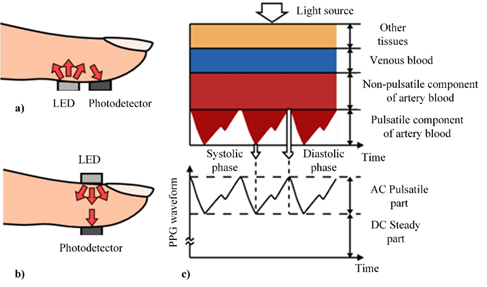
\includegraphics[width=0.7\linewidth]{img/PPG.png}
    \caption{Partes de la señal PPG. Fuente:\cite{Dzedzickis2020}.}
    \label{fig:PPG}
\end{figure}

Durante la sístole, el corazón bombea sangre hacia las arterias, aumentando el volumen sanguíneo en los capilares del área donde está colocado el sensor PPG. Como hay más sangre arterial, la absorción de luz infrarroja y roja aumenta, lo que reduce la intensidad de la luz detectada por el fotodetector. En la señal PPG, esto se observa como un pico (máxima amplitud).

Durante la diástole (relajación del corazón), el volumen sanguíneo en los capilares disminuye porque la sangre fluye de regreso al corazón. Al haber menos sangre arterial, la absorción de luz disminuye y más luz llega al fotodetector. En la señal PPG, esto se observa como un valle (mínima amplitud).


Esta señal es la base de la que partimos en el proyecto, y hablaremos sobre su tratamiento en la sección \ref{cap: Metodología}.

\subsection{Aplicación: El pulsioxímetro}

Todo lo expuesto hasta ahora se materializa en un dispositivo compacto y portátil: el pulsioxímetro. Este instrumento permite monitorizar en tiempo real la saturación de oxígeno y la frecuencia cardíaca del paciente, de forma continua y no invasiva. 

Está compuesto por un sensor con un diodo emisor de luz roja e infrarroja (LED) y un fotodiodo detector, los cuales están conectados al oxímetro (monitor) mediante un cable. El sensor mide cuánta luz de cada longitud de onda llega al fotodetector y, a partir de ahí, se calcula un cociente que se relaciona con la proporción de hemoglobina oxigenada.

\begin{figure}[H]
    \centering
    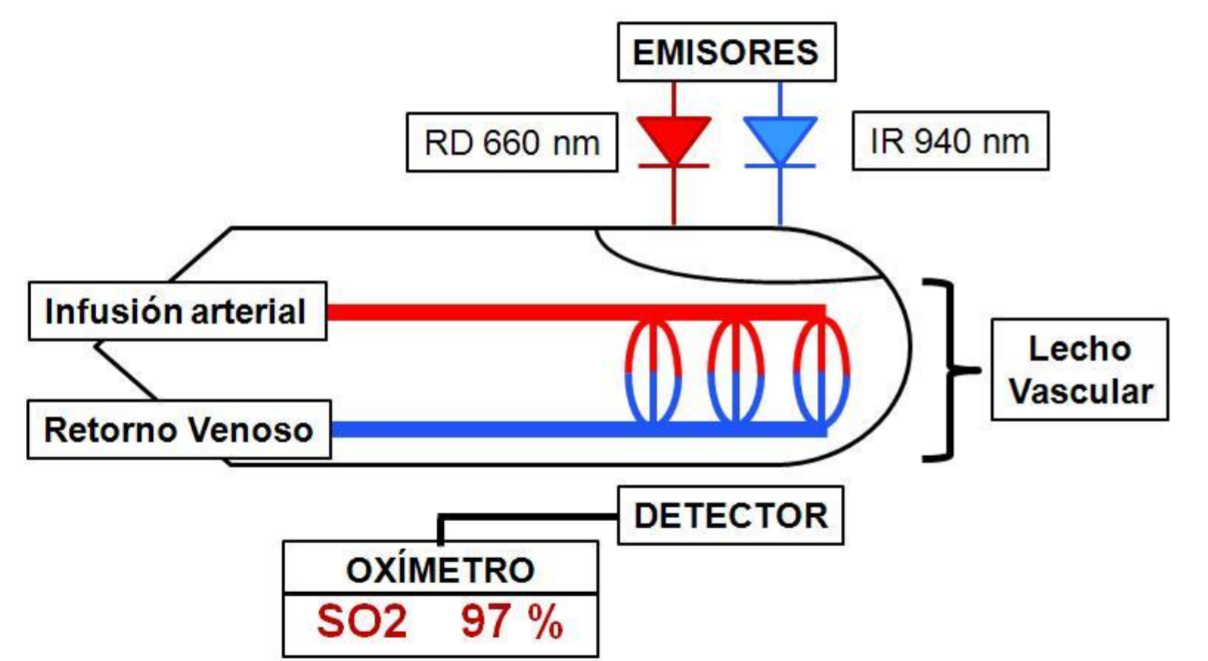
\includegraphics[width=0.6\linewidth]{img/pulsioximetrofuncionamiento.png}
    \caption{Esquema de funcionamiento y partes de un pulsioxímetro.
    \\ Fuente: \cite{medicinajoven_pulsioximetro}. }
    \label{fig:pulsioximetro}
\end{figure}

A medida que la luz pasa a través de la sangre pulsátil, la hemoglobina absorbe una de las longitudes de onda y deja pasar la otra, dependiendo de su estado de oxigenación. Cuando la hemoglobina está unida al oxígeno, refleja la luz roja y absorbe la infrarroja, lo que le confiere un color rojo brillante. En ausencia de oxígeno, la hemoglobina absorbe la luz roja y refleja la infrarroja, adquiriendo un tono rojo oscuro \cite{imfesPulsioximetro2025}.\\

El sensor detecta estas variaciones debidas a los cambios en el volumen arterial y, mediante algoritmos de calibración basados en datos experimentales, el dispositivo determina la proporción relativa de hemoglobina oxigenada en sangre y calcula automáticamente los valores de SpO$_2$\footnote{A partir de este punto se empleará el término \textbf{SpO$_2$}, que hace referencia a la saturación periférica de oxígeno estimada mediante pulsioximetría, en lugar de \textbf{SaO$_2$}, que corresponde a la saturación arterial medida de forma invasiva mediante análisis de gases en sangre. Aunque no son equivalentes, la SpO$_2$ se utiliza como una aproximación clínica habitual de la SaO$_2$.}
 y frecuencia cardíaca.

La señal PPG del pulsioxímetro se puede obtener a través de dos configuraciones del sensor:

\begin{itemize}
    \item \textbf{Reflectiva:} Ambos componentes (LED y fotodetector) están en el mismo lado.
    \item \textbf{Transmisiva :} Se usa cuando el LED y el fotodetector están en lados opuestos del tejido (ej., en un lóbulo de la oreja o el dedo).
\end{itemize}

En la parte práctica, utilizamos un sensor de tipo transmisivo, en el que la luz atraviesa el tejido antes de ser captada por el fotodetector.


\subsubsection{Factores que pueden afectar a la medición }

En muchos casos, las mediciones de los pulsioxímetros en atención médica pueden verse afectadas por varias circunstancias:

\begin{itemize}
\item \textbf{Movimiento}

El movimiento es una de las principales fuentes de error en la medición de SpO$_2$, especialmente en recién nacidos. La oximetría de pulso convencional asume que solo la sangre arterial presenta un componente pulsátil, pero el movimiento también genera variaciones ópticas y desplazamiento de sangre venosa. Esto puede hacer que el pulsioxímetro interprete erróneamente la señal venosa como arterial, reduciendo la precisión de la medición y generando valores falsamente bajos.

\item \textbf{Baja perfusión}

Cuando la perfusión disminuye (por hipotermia o bajo gasto cardíaco), la señal pulsátil se reduce y puede acercarse al nivel de ruido del pulsioxímetro. En casos extremos, la señal fisiológica queda enmascarada, afectando la precisión de la medición. 

\item \textbf{Interferencias externas}

\begin{itemize}
    \item Pigmentación de la piel: La piel oscura y ciertos esmaltes absorben luz a 660 nm y 940 nm, afectando la medición de SpO$_2$ en niveles bajos. 
    \item Interferencia electromagnética: Equipos como tomógrafos, aparatos quirúrgicos eléctricos o teléfonos móviles pueden alterar la lectura y causar sobrecalentamiento del sensor. 
    \item Luz ambiental: La exposición a luces intensas (quirófano, fototerapia) puede interferir con la lectura.
\end{itemize}


\item \textbf{Variantes de hemoglobina}

\begin{itemize}
    \item Carboxihemoglobina (COHb): Puede sobreestimar la SpO$_2$ en pacientes expuestos al monóxido de carbono, como fumadores o intoxicados. 
    \item Metahemoglobina: En casos de intoxicación por fármacos o anestésicos, altera la absorción de luz y genera mediciones imprecisas. 
\end{itemize}

\item \textbf{Oximetría de pulso en altura}

A nivel del mar, la SpO$_2$ normal es 97-99\% (límite inferior: 94\%). A mayores altitudes (>2500 msnm), la presión de oxígeno disminuye, adaptando los niveles de SpO$_2$. En niños sanos que residen en altura, valores entre 85-87\% pueden considerarse normales. \cite{oximetria_pulso2012}

\end{itemize}

\section{Procesamiento Digital de Señales Biomédicas}

Después de haber explicado en qué consiste la pulsioximetría, el siguiente paso es entender cómo se trabaja con las señales que genera el sensor. Estas señales, aunque contienen información relevante, no siempre son claras ni fáciles de interpretar.

El organismo se comunica consigo mismo a través de señales de diversa naturaleza, que en el cuerpo humano se reducen a la energía eléctrica, química, mecánica y térmica. Estas señales biomédicas contienen información valiosa sobre los procesos fisiológicos, aunque dicha información no siempre es perceptible. En muchos casos, la información útil se encuentra oculta en la estructura de la señal, requiriendo ser decodificada o extraída mediante técnicas adecuadas de análisis \cite{carrion2011procesado}.


\begin{table}[H]
\centering
\begin{tabular}{|l|p{5cm}|p{6cm}|}
\hline
\textbf{Energía} & \textbf{Variables} & \textbf{Mediciones} \\
\hline
Química   & Concentración química & Concentraciones en sangre, O$_2$, CO$_2$, pH, hormonas, etc. \\ \hline
Mecánica  & Posición, torque, presión & Contracción muscular, presión cardiovascular, sonidos cardíacos, etc. \\\hline
Eléctrica & Voltaje y corriente de flujo iónico & EEG, ECG, EMG, PPG \\\hline
Térmica   & Temperatura & Termografía clínica \\
\hline
\end{tabular}
\caption{Tipos de energía, variables biológicas asociadas y ejemplos de mediciones biomédicas. Fuente: \cite{dePedroCarracedo2020}.}
\label{tabla:energia}
\end{table}


Las señales biomédicas reflejan propiedades intrínsecas de los sistemas biológicos de los que provienen, y su estudio permite identificar tanto estados normales como patológicos. En algunas situaciones, una simple inspección visual de la señal puede ser suficiente para interpretar su contenido; sin embargo, la complejidad de la mayoría de las señales fisiológicas hace necesario aplicar técnicas de procesamiento digital, que permitan extraer de forma fiable la información clínica relevante.

\subsection{Adquisición de señales biomédicas}

El procesamiento de señales biomédicas comienza con su correcta adquisición. Esta consiste en transformar una señal analógica, continua en el tiempo, en una representación digital adecuada para el tratamiento numérico. Este proceso implica el desarrollo de varias etapas:

\begin{itemize}
    \item \textbf{Captura de la señal: }mediante sensores que convierten la magnitud biológica en una señal eléctrica proporcional, por ejemplo, la absorción de luz en PPG.
    \item \textbf{Acondicionamiento}: puede incluir amplificación, filtrado analógico inicial y adaptación de la señal al rango dinámico del conversor analógico-digital (ADC).
    \item \textbf{Conversión analógico-digital (ADC):} que consiste en la discretización temporal mediante muestreo periódico y la discretización en amplitud mediante cuantificación.
\end{itemize}

Para conservar la información contenida en la señal original, el teorema de Nyquist establece que la frecuencia de muestreo debe ser, al menos, el doble de la máxima frecuencia presente en la señal. En señales de interés fisiológico, como las captadas mediante PPG, la frecuencia de muestreo suele situarse entre 50 y 200 Hz, dependiendo de la aplicación concreta.

En el caso de este proyecto, la fase de adquisición de la señal ha supuesto una gran parte del desarrollo, que se explicará en la sección \ref{cap: Metodología}.

\subsection{Filtrado digital de señales}

Es habitual que las señales, una vez adquiridas, contengan no solo la información fisiológica de interés, sino también componentes de ruido e interferencias no deseadas. El objetivo del filtrado digital es eliminar o atenuar estas perturbaciones sin distorsionar el contenido útil de la señal. Para ello, es necesario que las características del filtro se ajusten al espectro de interés. En aplicaciones biomédicas, este espectro puede variar en función del tipo de señal, del estado fisiológico del paciente y de la calidad de adquisición, lo que justifica la necesidad de adaptar los parámetros del filtro a cada caso particular \cite{studysmarter_filtro_biosenales}.

Según las necesidades del análisis, pueden emplearse distintos tipos de filtros:

\subsubsection{Según la función que realizan}

\textbf{Filtros paso bajo}

Permiten el paso de señales por debajo de una frecuencia de corte y atenúan señales por encima de la frecuencia de corte. Es decir, eliminan las componentes de alta frecuencia, como el ruido eléctrico o artefactos \cite{mathworks_lowpass_filter}.

\textbf{Filtros paso alto}

Los filtros paso alto atenúan las señales situadas por debajo de una frecuencia de corte y permiten el paso de señales situadas por encima de la frecuencia de corte. Es decir, eliminan componentes de muy baja frecuencia, como el desplazamiento de la línea base \cite{mathworks_highpass_filter}.

\textbf{Filtros paso banda}

Permiten seleccionar el rango de frecuencias donde se encuentra la información de interés, atenuando o bloqueando las frecuencias fuera de ese rango \cite{rubia2021diseno}.

\textbf{Filtros IIR (Infinite Impulse Response) }

Los filtros IIR (Respuesta Infinita al Impulso) son filtros digitales cuya respuesta al impulso teóricamente se extiende indefinidamente, ya que utilizan tanto valores pasados de la señal de entrada como de la salida filtrada \cite{gonzalez2014filtrado}, esto les permite lograr ciertos efectos de filtrado usando menos cálculos que otros filtros.

\textbf{FIR (Finite Impulse Response)}

Los filtros FIR (Respuesta Finita al Impulso) son filtros digitales cuya respuesta al impulso tiene una duración limitada en el tiempo, ya que dependen exclusivamente de valores actuales y pasados de la señal de entrada. Son estables y pueden diseñarse para tener una respuesta de fase lineal \cite{gonzalez2014filtrado}.

En la figura \ref{fig:filtros} se puede observar cómo modifica cada filtro a la señal.

\begin{figure}[H]
    \centering
    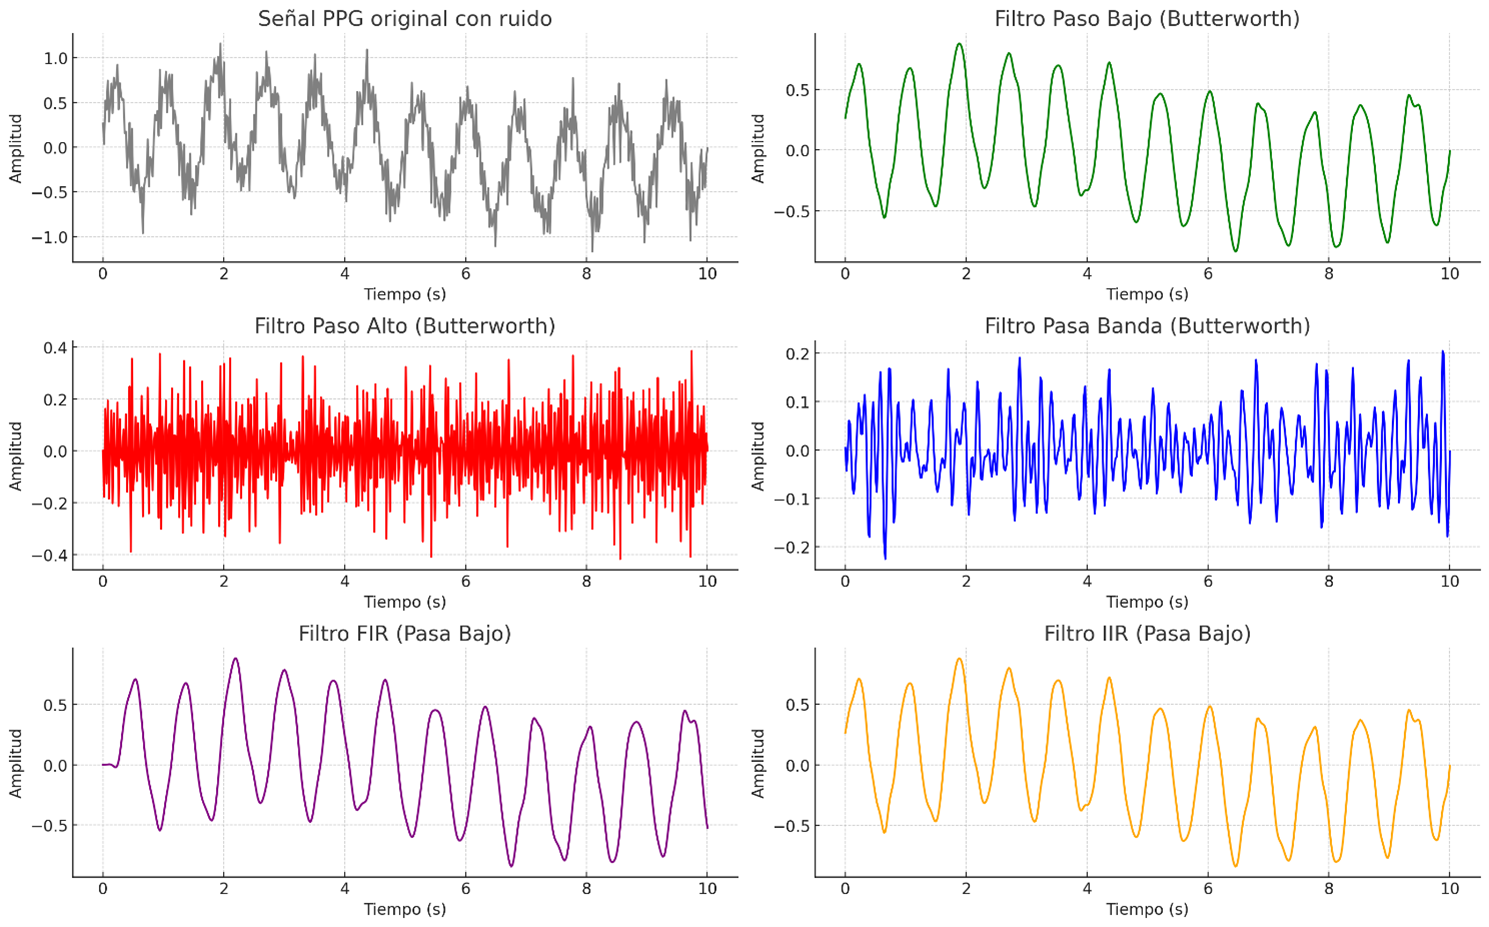
\includegraphics[width=0.92\linewidth]{img/filtros.png}
    \caption{Comparación de los tipos de filtrado mencionados a partir de una señal PPG. \textit{Elaboración propia}.}
    \label{fig:filtros}
\end{figure}

\subsubsection{Según el diseño o implementación}

\textbf{Moving Average o filtro de media móvil}

Se utiliza para suavizar las señales adquiridas. Consiste en reemplazar cada muestra de la señal por el promedio de un número fijo de muestras adyacentes. Se trata de un método simple y computacionalmente eficiente para suavizar variaciones rápidas y aleatorias en la señal. Sin embargo, puede distorsionar transiciones rápidas o picos pronunciados \cite{mathworks_lowpass_filter}.

\textbf{Filtro de Savitzky-Golay}

Este método suaviza la señal mediante un ajuste polinomial local de las muestras. A diferencia de la media móvil, el filtro de Savitzky-Golay conserva mejor la forma y amplitud de las características locales de la señal, como picos o valles, haciendo que sea especialmente útil en señales donde es importante preservar la morfología.

\textbf{Filtro Butterworth}

Los filtros de Butterworth se caracterizan por una respuesta en frecuencia plana en la banda pasante, lo que significa que no introduce oscilaciones ni altera la forma original de la señal. Además, su transición hacia la zona donde se atenúan las frecuencias no deseadas (banda de corte) es suave y progresiva, lo que ayuda a reducir el ruido sin introducir artefactos bruscos. Es una buena opción cuando se quiere mantener la señal lo más parecida posible a la original, pero más limpia.

\begin{figure}[H]
    \centering
    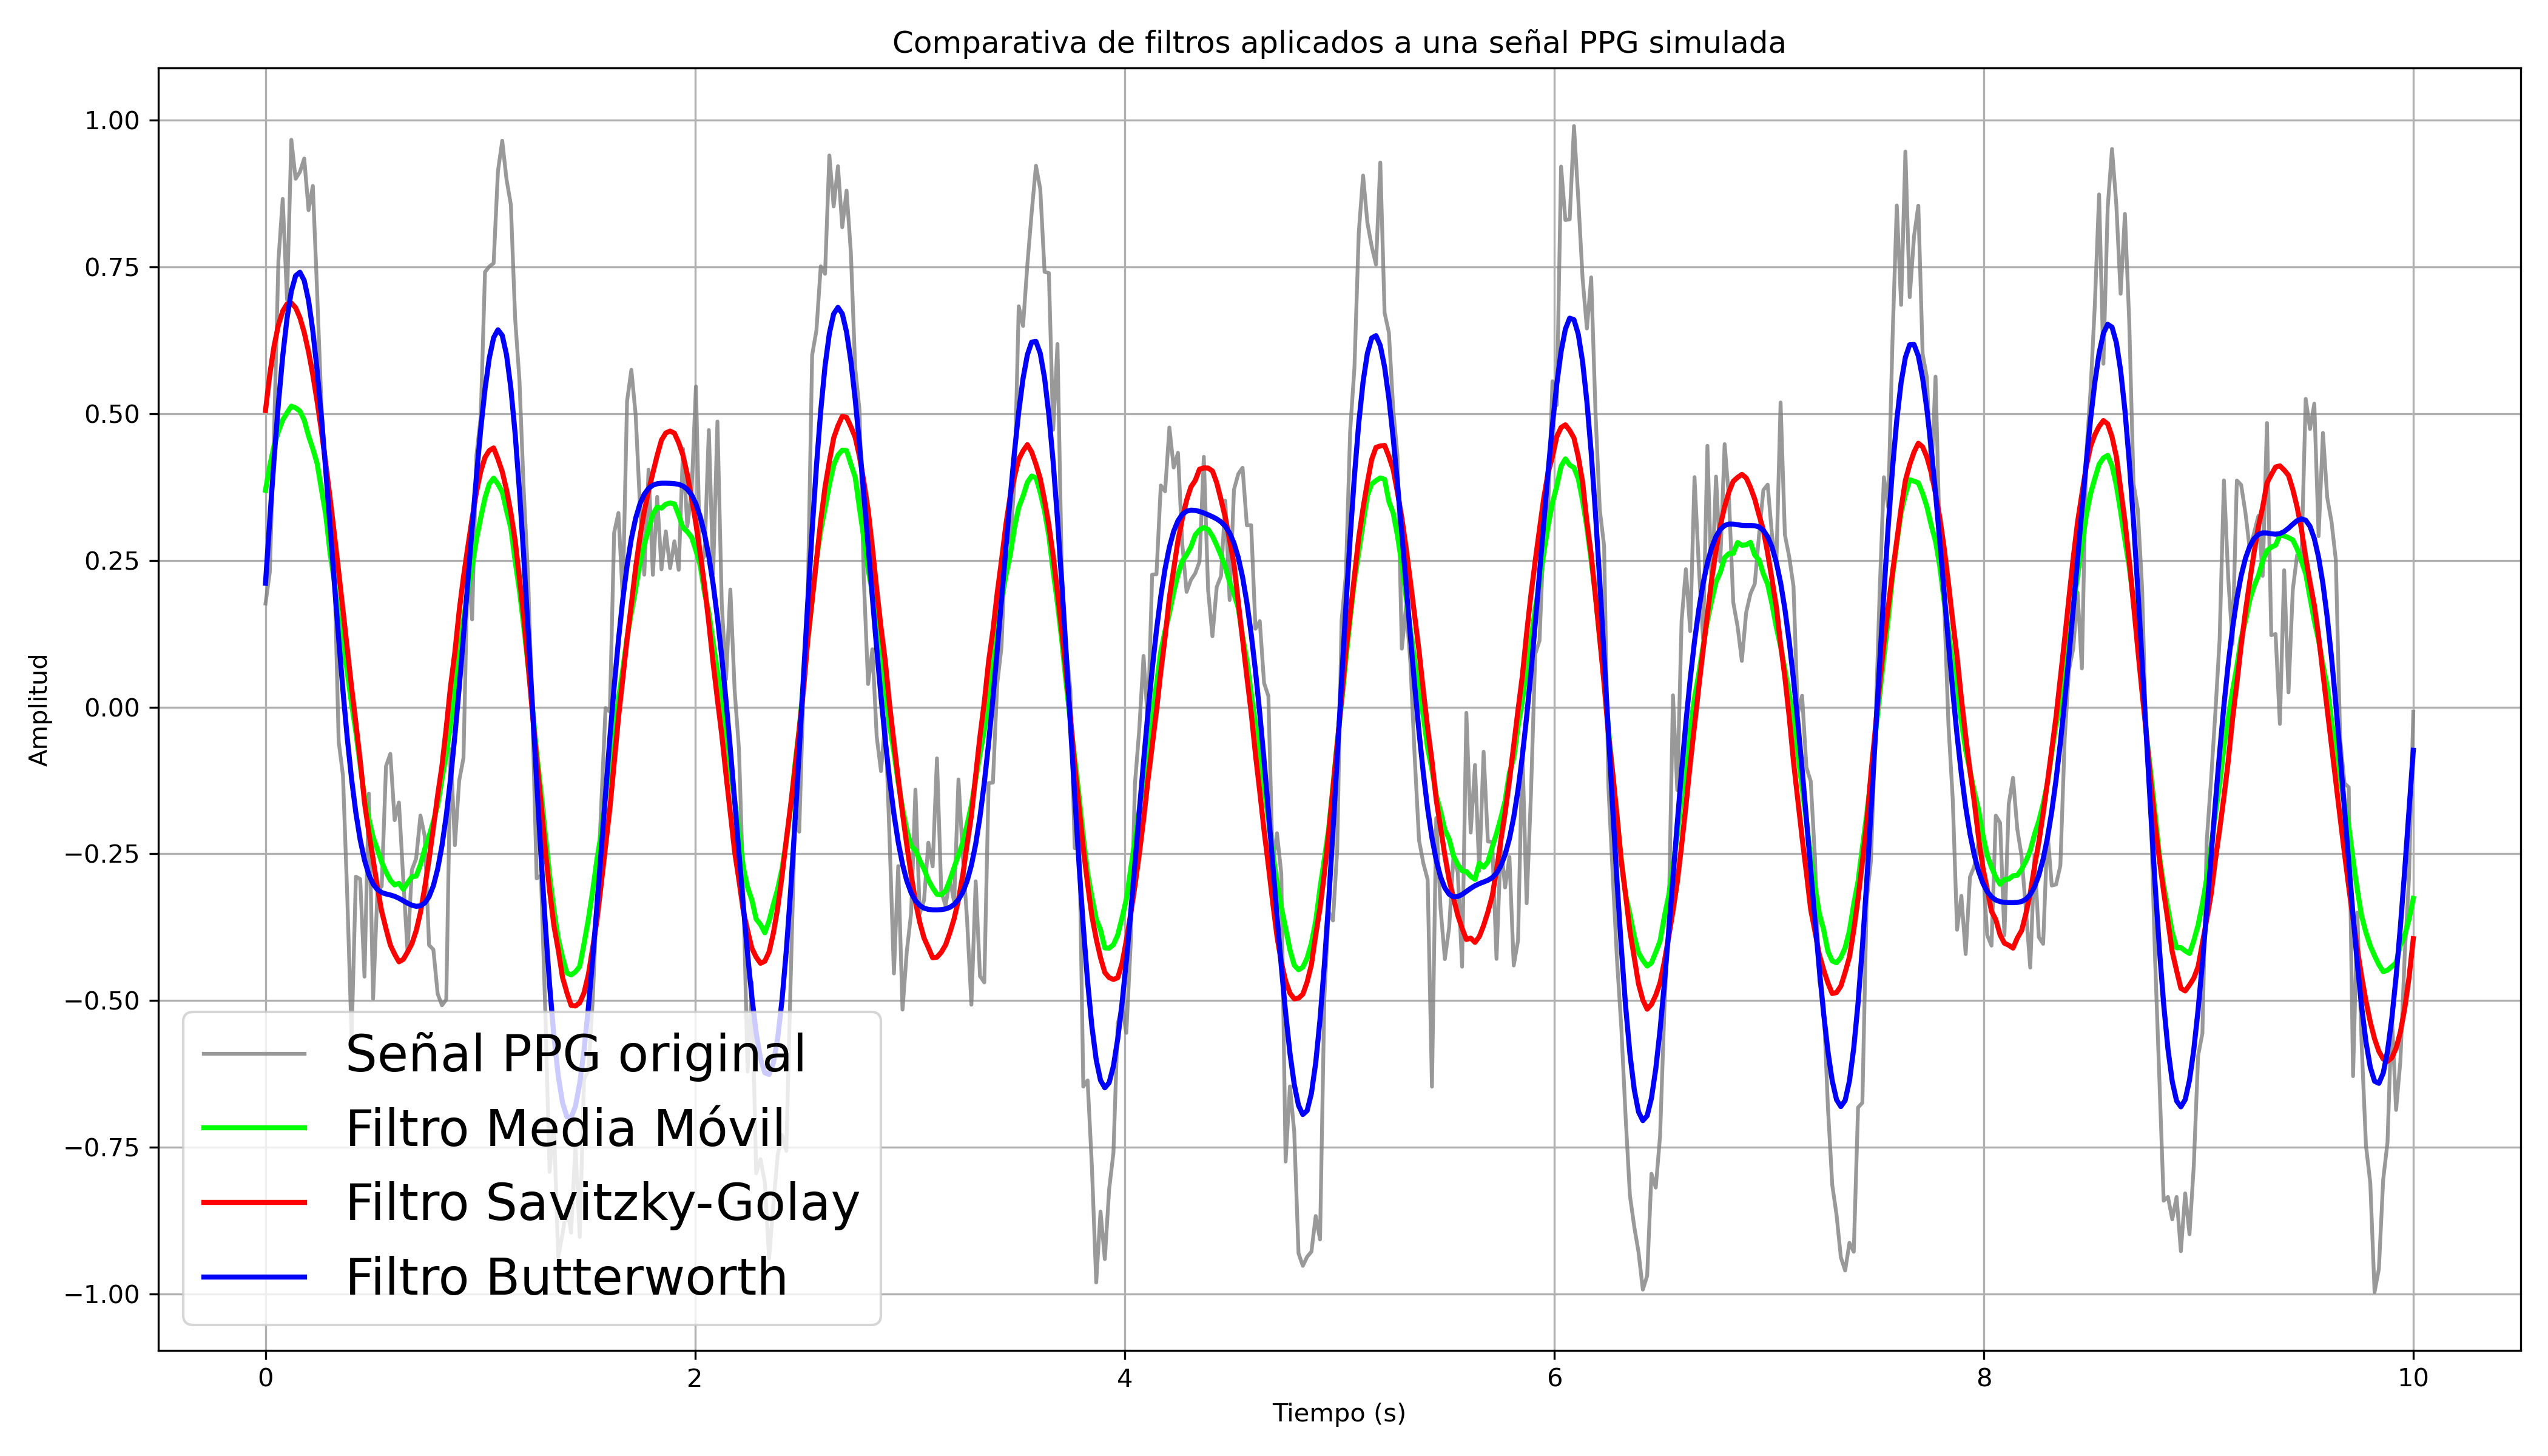
\includegraphics[width=0.85\linewidth]{img/filtrados.png}
    \caption{Comparación de los tipos de filtros según el diseño o implementación. \textit{Elaboración propia}.}
    \label{fig:filtrados}
\end{figure}

Solo se han descrito aquellos filtros que han sido implementados en este trabajo, omitiendo otros tipos cuya aplicación no ha sido necesaria para los objetivos planteados.

\subsection{Modelos y Algoritmos para la Conversión de Señales en Parámetros Clínicos}

Para que un pulsioxímetro proporcione información útil, es necesario transformar las señales ópticas captadas, en parámetros fisiológicos interpretables por un ser humano. Esta conversión se basa en modelos matemáticos y algoritmos de procesamiento de señal que permiten extraer información fiable. A continuación, se describen los fundamentos y métodos empleados para el cálculo de ambos parámetros.

\subsubsection{Cálculo de la Frecuencia Cardíaca:}

En los pulsioxímetros comerciales, la frecuencia cardíaca se estima a partir de la señal PPG, que refleja las variaciones en el volumen de sangre generadas por cada latido del corazón. Estas oscilaciones, visibles como picos en la señal, permiten identificar el momento en que ocurre cada pulso arterial.

\begin{figure}[H]
    \centering
    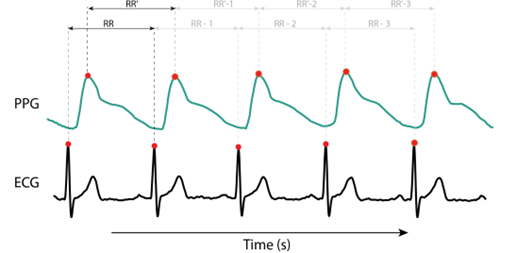
\includegraphics[width=0.75\linewidth]{img/ECGvsPPG.png}
    \caption{Comparación entre señales PPG y ECG para la medición del intervalo RR. 
    \\ Fuente: \cite{vandenberk2017fibricheck}.}
    \label{fig:ECGvsPPG}
\end{figure}

El primer paso del algoritmo suele ser aplicar un filtro para aislar el rango de frecuencias correspondiente a la actividad cardíaca, eliminando así componentes no deseadas como el ruido de alta frecuencia o las variaciones lentas del entorno \cite{liu2021wearable}.

Posteriormente, se realiza una detección de picos, normalmente sobre la componente AC de la señal infrarroja. Cada pico representa un latido cardíaco. 

A partir del intervalo temporal entre picos sucesivos (intervalos RR), se calcula la frecuencia cardíaca mediante la ecuación \ref{eq: HR}:

\begin{equation}
\text{HR (BPM)} = \frac{60}{\text{intervalo entre picos (s)}}
\label{eq: HR}
\end{equation}



Para evitar oscilaciones en la lectura, algunos dispositivos promedian el intervalo entre varios picos consecutivos. La estabilidad del cálculo depende de la calidad de la señal y del rendimiento del algoritmo de detección, que debe ser robusto frente a artefactos de movimiento o presión inadecuada del sensor.

\subsubsection{Cálculo de la Saturación de Oxígeno (SpO\textsubscript{2})}

Tal y como se ha explicado con anterioridad, la estimación de la saturación de oxígeno en sangre mediante pulsioximetría se basa en la Ley de Beer-Lambert, con la que se logra definir que la intensidad de la luz disminuye con la longitud de la trayectoria, siendo conocedores de que la señal de la luz transmitida a través del dedo está formada por una componente de corriente continua (DC) y una de corriente alterna (AC) \cite{liu2021wearable}. 

A partir de estas componentes, se calcula el \textbf{Ratio R} (\ref{eq:ratio}) característico:

\begin{equation}
    R = \frac{\frac{\mathrm{AC}_{\text{red}}}{\mathrm{DC}_{\text{red}}}}{\frac{\mathrm{AC}_{\text{IR}}}{\mathrm{DC}_{\text{IR}}}}
    \label{eq:ratio}
\end{equation}

El valor de \( R \) se relaciona experimentalmente con el porcentaje de saturación de oxígeno mediante una curva de calibración (figura \ref{fig:ratio}), obtenida mediante estudios en voluntarios sanos. Dado que resulta peligroso inducir saturaciones muy bajas (por debajo del 75\%), los pulsioxímetros extrapolan la calibración en ese rango mediante modelos matemáticos.

\begin{figure}[H]
    \centering
    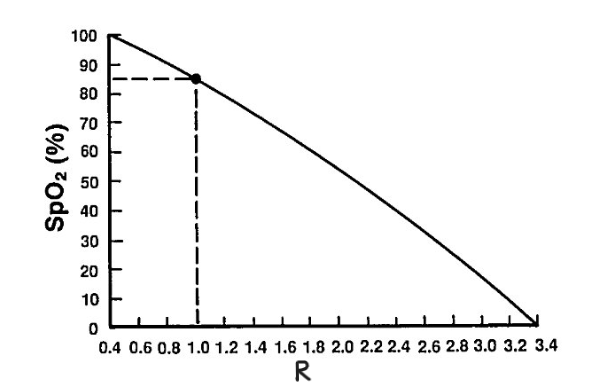
\includegraphics[width=0.55\linewidth]{img/ratio.png}
    \caption{Explicación gráfica del cálculo de la SpO$_2$ a partir de R. Fuente adaptada: \cite{deshmane2009false}.}
    \label{fig:ratio}
\end{figure}

La relación empírica adoptada por muchos dispositivos comerciales puede aproximarse mediante una ecuación lineal (\ref{eq: spo2_3}) del tipo:

\begin{equation}
    \text{SpO}_2 (\%) = A - (B \times R)
    \label{eq: spo2_3}
\end{equation}

donde \( A \) y \( B \) son constantes de calibración específicas de cada dispositivo. Por ejemplo, algunas implementaciones proponen valores como \( A = 110 \) y \( B = 25 \).

Además, para mejorar la estimación de SpO\textsubscript{2} en condiciones de baja perfusión o presencia de artefactos de movimiento, se utilizan técnicas de procesamiento digital adicionales como la \textit{Transformada Rápida de Fourier (FFT)} \cite{jimenez2019pulsioximetro}.


\section{Estado del arte y trabajos relacionados}

Se presenta a continuación una recopilación de desarrollos recientes vinculados a esta tecnología, seleccionados por su interés particular para este proyecto.

\subsection{Dispositivos comerciales y soluciones de bajo coste}

Los pulsioxímetros comerciales ofrecen alta precisión, pero su elevado coste limita su integración o adquisición en entornos con recursos limitados. Como alternativa, han surgido múltiples proyectos open-source y de bajo coste basados en sensores como el MAX30102, integrables en plataformas como Arduino \cite{llamas_pulsimetro_max30102}. 

Iniciativas como \textbf{OpenOximetry.org} \cite{openoximetry2025} proponen estándares abiertos para mejorar la precisión y validación de pulsioxímetros en contextos desfavorecidos.

\begin{figure}[H]
    \centering
    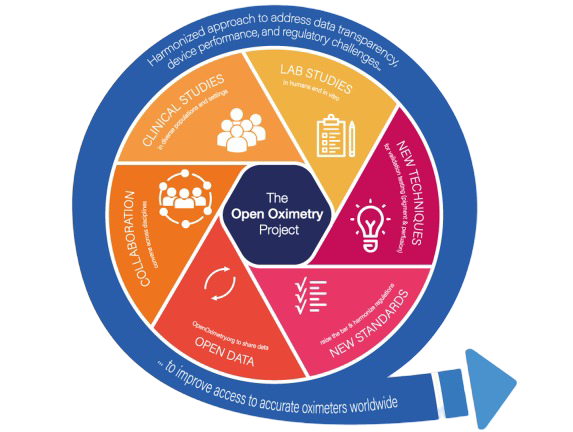
\includegraphics[width=0.6\linewidth]{img/openoximetry.png}
    \caption{Esquema del enfoque y objetivo del Open Oximetry Project. Fuente: \cite{elmankabadi2023openoximetry}.}
    \label{fig:openoximetry}
\end{figure}

\subsection{Aplicaciones en salud global y neonatología}

Durante la pandemia de COVID-19, la pulsioximetría se popularizó para el monitoreo domiciliario. En neonatología, se propone su uso para detectar afecciones frecuentes como la hipoxia o las cardiopatías congénitas. La Global Oximetry Initiative \cite{thoms2007global}, por ejemplo, es una iniciativa lanzada en el año 2007 en Uganda, India, Filipinas y Vietnam, cuyo objetivo principal es promover el uso de la oximetría y reducir sus costos en países de bajos ingresos, así como la creación de nuevas políticas, influir en su diseño y establecer nuevos estándares globales para una monitorización más segura.


\subsection{Proyectos relacionados}

Se han desarrollado numerosos prototipos de la solución tecnológica propuesta. Se mencionan brevemente los que se han considerado más relevantes: 

\begin{itemize}
    \item \textbf{Diseño y simulación de un pulsioxímetro a bajo costo}: Este proyecto de tesis propone un pulsioxímetro económico utilizando un Arduino Uno, con el objetivo de disminuir su costo en un 15\% y fomentar su fabricación local en Honduras para áreas de enfermería de CEUTEC \cite{chacon2021pulsioximetro}.
    \item \textbf{Diseño e implementación de un pulsioxímetro reflexivo y estudio de su funcionamiento en diferentes zonas del cuerpo :} Este trabajo de fin de grado se centra en el diseño de un prototipo de pulsioxímetro reflexivo utilizando el sensor MAX30102 y un microprocesador, evaluando su precisión y viabilidad para aplicaciones médicas \cite{gonzalez2019pulsioximetro}.
    \item \textbf{Pulsioxímetro con registro de datos en IoT y generación de alertas}: Este TFG propone un pulsioxímetro económico con comunicación Wi-Fi para registrar datos de frecuencia cardíaca y saturación de oxígeno en la nube mediante ThingSpeak\footnote{ThingSpeak es una plataforma de análisis de IoT que permite agregar, visualizar y analizar flujos de datos en vivo en la nube}, permitiendo generar alertas automáticas. Utiliza el sensor MAX30100 y un ESP8266 como microcontrolador \cite{sein2019pulsioximetro}.
    \item \textbf{Diseño e implementación de un pulsioxímetro orientado a deportistas de apnea}: Este proyecto desarrolla un prototipo básico de pulsioxímetro con fines deportivos, con especial atención a las condiciones de presión y temperatura extremas. Utiliza Arduino y sensores ópticos específicos, y propone mejoras de diseño para su aplicación subacuática \cite{borbones2021pulsioximetro}.
    \item \textbf{Medida del nivel de saturación de oxígeno en sangre: desarrollo de un pulsioxímetro de bajo coste y comparativa con otros sistemas existentes}: Este trabajo desarrolla un pulsioxímetro de bajo coste basado en la Ley de Beer-Lambert, usando sensores ópticos para estimar SpO$_2$ de forma no invasiva \cite{Alarco2015}.
    \item \textbf{Diseño de un pulsioxímetro de bajo coste y salida bluetooth}: Presenta el diseño e implementación de un pulsioxímetro económico que transmite datos de SpO$_2$ y pulso vía Bluetooth, orientado a su uso en telemedicina \cite{jimenez2019pulsioximetro}.
\end{itemize}


\subsection{Algoritmos de estimación de la frecuencia cardíaca}

También se ha investigado acerca de los diferentes enfoques que se han propuesto para la estimación de la frecuencia cardíaca a partir de señales PPG:

\begin{itemize}
  \item \textbf{Detección de picos en el dominio temporal:} como se ha mencionado, se trata del método más clásico y utilizado. Fue analizado por Elgendi \cite{elgendi2012analysis} y optimizado por Vourvoulakis et al. \cite{9493400} mediante un umbral adaptativo y ventanas deslizantes para mejorar la robustez.

  \item \textbf{Método de cruce de umbral (Threshold-Crossing):} Este algoritmo detecta cuándo la señal cruza un umbral dinámico derivado del nivel de señal. Incluye un mecanismo de \textit{debounce}\footnote{técnica que se utiliza para evitar que se activen falsas pulsaciones o cambios de estado debido a rebotes mecánicos o eléctricos en dispositivos electrónicos} para evitar el doble conteo de un mismo latido. Es simple y rápido, aunque puede verse afectado por ondas dicrotas\footnote{La onda dícrota es una pequeña depresión o muesca que aparece en la pendiente descendente de la onda de presión arterial} o ruido de movimiento \cite{renesas2022ob1203}.

  \item \textbf{Análisis en el dominio de la frecuencia:} Consiste en aplicar una Transformada Rápida de Fourier (FFT) sobre un fragmento de la señal PPG para identificar su frecuencia dominante. Este método es útil cuando la señal es estable y periódica, pero menos fiable en presencia de ruido o no estacionariedad \cite{electronics3020282}.

  \item \textbf{Aprendizaje automático (ML):} Modelos como Random Forest o redes neuronales convolucionales (CNN) permiten estimar la HR extrayendo automáticamente características relevantes de la señal. Estos modelos han demostrado ser robustos frente a artefactos de movimiento y ruido fisiológico \cite{biswas2019cornet}.

  \item \textit{\textbf{Rapid, remote and low-cost finger vasculature mapping for heart rate monitoring: }}Este estudio presenta una metodología para mapear la vasculatura del dedo y monitorear la frecuencia cardíaca de manera remota y económica, utilizando equipos disponibles comercialmente y algoritmos de procesamiento de imágenes \cite{kallepalli2022finger}.
\end{itemize}


\subsection{Algoritmos de estimación de la saturación de oxígeno}

Del mismo modo, se han revisado estudios que utilizan distintos métodos para estimar la saturación de oxígeno en sangre a partir de señales PPG. Aunque la mayoría de ellos se basa en el enfoque del \textit{Ratio of Ratios}, mencionado anteriormente, también existen otras propuestas que buscan mejorar la precisión o adaptarse mejor a diferentes condiciones:


\begin{itemize}
  \item \textbf{Compresión de muestras (Compressed Sensing):} Se utilizan señales submuestreadas por debajo de la tasa de Nyquist para estimar SpO$_2$, lo que permite reducir el consumo energético sin pérdida significativa de precisión. Es útil en dispositivos portátiles o wearable \cite{mohan2010blood}.

  \item \textbf{Aprendizaje automático:} Modelos basados en redes neuronales profundas pueden aprender directamente la relación entre la señal PPG cruda y los valores reales de SpO$_2$. Estos métodos han mostrado alta precisión incluso con señales degradadas por artefactos de movimiento\cite{shuzan2023machine}.
\end{itemize}
